Para el actual proyecto se necesita un groupware al cu\'al se le pueda acoplar la arquitectura, en este caso el sistema elegido es un video juego colaborativo de disparos en primera persona, \textit{AssaultCube}. Este groupware en particular tiene las caracter\'isticas de ser distribuido y s\'incrono seg\'un la clasificaci\'on de Ellis\cite{ellis1991groupware}, contiene varios tipos de elementos y los modos multijugador son entre equipos en los cuales se requiere de una buena colaboraci\'on para cumplir los objetivos de la actividad, El juego cuenta con un servidor y varios clientes que se conect\'an a \'el para jugar, la arquitectura tendr\'a que estar acoplada al servidor ya que este es el que recibe toda la informaci\'on de las actividades de los clientes.

El servidor del video juego \textit{Assault Cube} est\'a desarrollado para la plataforma Linux, el cliente para Windows, y la arquitectura a desarrollar ser\'a programada en C\#. \textit{Assault Cube} tiene diferentes modos de juego, entre ellos capturar la bandera, cuyo objetivo es llegar a la base enemiga y recuperar la bandera que est\'a ah\'i para regresarla a la propia bas; otro modo de juego es rey de la colina, que tiene por objetivo mantenerse m\'as tiempo en una posici\'on marcada por el juego que el equipo contrario; hay m\'as formas de juego adem\'as de estas dos, y en cada una de ellas las actividades son diferentes y poseen objetivos diferentes, sin embargo pueden compartir interacciones como eliminar a un enemigo por ejemplo.

\begin{figure}[h!]
\centering
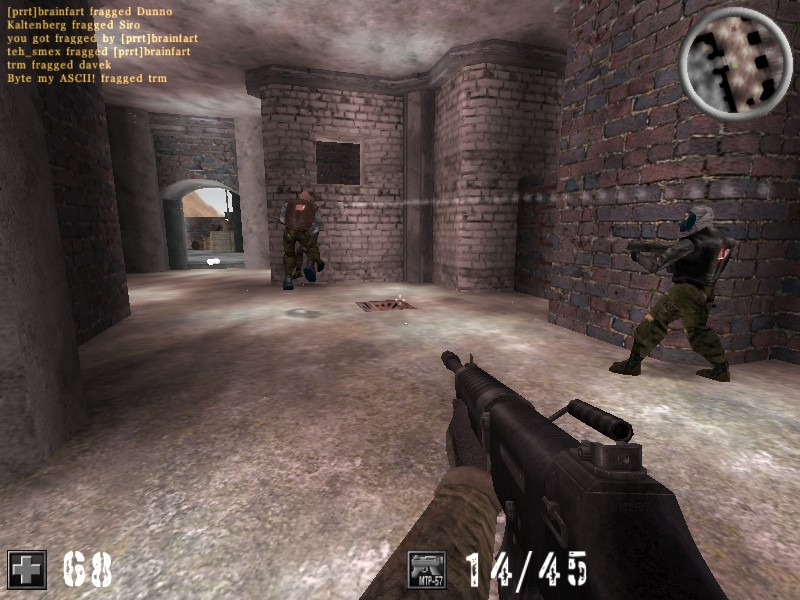
\includegraphics[scale=.20]{images/assaultcube}
\caption{Assault Cube}
\label{gw:asscb}
\end{figure}

En el Cuadro \ref{sc:interacciones} se muestran las interacciones identificadas en el juego para la actividad relacionada al modo de juego de capturar la bandera, estas interacciones est\'an relacionadas directamente con las actividades que se pueden llevar a cabo en el groupware, las interacciones se vuelven irrelevantes cuando no tienen conexi\'on con ninguna actividad, por ejemplo las interacciones del usuario con elementos de configuraci\'on en este caso particular, como en la interacci\'on \textit{"Jugador elige modo de juego"}. En estas interacciones se encuentran algunos elementos del modelo como pueden ser Actores, Tareas y Objetos,  esto nos da la pauta para empezar a dise\~nar nuestro modelo.

\begin{center}
\label{sc:interacciones}
\begin{longtable}{|p{5cm}|p{7cm}|}

\caption{Interacciones detectadas en \textit{Assault Cube}}\\
\hline
\textbf{Interacci\'on} & \textbf{Elementos identificados}\\
\hline
\endfirsthead
\multicolumn{2}{c}%
{\tablename\ \thetable\ -- \textit{... Contin\'ua de p\'agina anterior}} \\
\hline
\textbf{Interacci\'on} & \textbf{Elementos identificados} \\
\hline
\endhead
\hline \multicolumn{2}{r}{\textit{Contin\'ua en siguiente p\'agina...}} \\
\endfoot
\hline
\endlastfoot
\textbf{Jugador se Mueve} & Actor: Jugador; Tarea: Moverse\\\hline

\textbf{Jugador salta} & Actor: Jugador; Tarea: Saltar\\\hline

\textbf{Jugador dispara arma} & Actor: Jugador; Tarea: Saltar; Objeto: Arma\\\hline

\textbf{Jugador recarga arma} & Actor: Jugador; Tarea: Recargar; Objeto: Arma\\\hline

\textbf{Jugador dispara arma} & Actor: Jugador; Tarea: Saltar; Objeto: Arma\\\hline

\textbf{Jugador cambia arma} & Actor: Jugador; Tarea: Cambiar; Objeto: Arma\\\hline

\textbf{Jugador obtiene mejora de salud} & Actor: Jugador; Tarea: Obtener; Objeto: Mejora de salud\\\hline

\textbf{Jugador obtiene protecci\'on} & Actor: Jugador; Tarea: Obtener; Objeto: Protecci\'on\\\hline

\textbf{Jugador obtiene munici\'on} & Actor: Jugador; Tarea: Obtener; Objeto: munici\'on\\\hline

\textbf{Jugador envia mensaje de texto} & Actor: Jugador; Tarea: enviar; Objeto: Mensaje de texto\\\hline

\textbf{Jugador envia mensaje de voz predefinido} & Actor: Jugador; Tarea: enviar; Objeto: Mensaje de voz\\\hline

\textbf{Jugador elige arma inicial} & Actor: Jugador; Tarea: Elegir; Objeto: Arma predeterminada\\\hline

\textbf{Jugador cambia rol} & Actor: Jugador; Tarea: Cambiar; Objeto: Rol\\\hline

\textbf{Jugador se agacha} & Actor: Jugador; Tarea: Agacharse\\\hline

\textbf{Jugador se suicida} & Actor: Jugador; Tarea: Suicidarse\\\hline

\textbf{Jugador es eliminado} & Actor: Jugador; Tarea: Ser eliminado\\\hline

\textbf{Jugador elimina oponente} & Actores: JugadorA, JugadorB; Tarea: Eliminar\\\hline

\textbf{Jugador reaparece} & Actor: Jugador; Tarea: Reaparecer\\\hline

\textbf{Jugador captura bandera} & Actor: Jugador; Tarea: Capturar; Objeto: Bandera\\\hline

\textbf{Jugador regresa bandera a su base} & Actor: Jugador; Tarea: Recuperar; Objeto: Bandera \\\hline

\textbf{Jugador ve mapa} & Actor: Jugador; Tarea: Ver; Objeto: Mapa\\\hline

\textbf{Jugador ve puntuaciones} & Actor: Jugador; Tarea: Ver; Puntuaciones\\\hline

\end{longtable}
\end{center}

En la lista anterior se pueden identificar ya algunos elementos del modelo del groupware, por ejemplo, jugador como actor; arma, munici\'on y mapa como posibles objetos, y el conjunto de ellos relacionados con una acci\'on como tareas. Adem\'as de los elementos identificados por medio de la observaci\'on, se explor\'o el sitio web oficial de la aplicaci\'on \cite{assCube2014} para extraer m\'as informaci\'on del juego. Se encontraron dos \textbf{comunidades}: team clubers liberation army(TCLA) y rabid viper special forces(RVSF) los que compiten uno en contra del otro en cada partida. Dos tipos de objetos, armas y art\'iculos, para las armas se describen atributos como tiempo de recarga, capacidad de munici\'on, rafaga de disparo, etc. Para los art\'iculos s\'olo se define el atributo de tiempo de reaparici\'on. Tambi\'en se identificaron objetivos seg\'un los tipos de partida, de los que se infieren algunas metas. En el cuadro \ref{sc:dominio} se muestran los elementos de dominio que se identificaron mediante la revisi\'on de la documentaci\'on del sistema.

\begin{center}
\label{sc:dominio}
\begin{longtable}{|p{3cm}|p{9cm}|}

\caption{Elementos de dominio de \textit{Assault Cube}}\\
\hline
\textbf{Elemento de Meta modelo} & \textbf{Elemento de dominio de la aplicaci\'on}\\
\hline
\endfirsthead
\multicolumn{2}{c}%
{\tablename\ \thetable\ -- \textit{... Contin\'ua de p\'agina anterior}} \\
\hline
\textbf{Elemento de Meta modelo} & \textbf{Elemento de dominio de la aplicaci\'on} \\
\hline
\endhead
\hline \multicolumn{2}{r}{\textit{Contin\'ua en siguiente p\'agina...}} \\
\endfoot
\hline
\endlastfoot

Actores & Jugador(p.ej. Juan, Ana, Marcos, etc.)\\
\hline Comunidades & Team Clubers Liberation Army (TCLA);
Rabid Viper Special Forces (RVSF).\\
\hline Objetos & Armas(Swiss tech cmbat blade DR-88, Mk-77 Semi-Automatic Pistol, MTP-57 Assault Rifle, Precision Tech AD-81 Sniper Rifle, A-ARD/10 Sub-machine Gun, V-19 Combat Shotgun, TMP-M\&A Carbine, SAL-T3 Grenade) , Art\'iculos(AmmoBox, Pistol Magazine, Akimbo, Healt, Helmet Armour, Kevlar Armour, Grenade). \\
\hline Roles & Explorer, Protector, Fragger, Recoverer.\\
\hline Objetivos & capturar la bandera, robar la bandera enemiga, eliminar jugadores enemigos, regresar la bandera a la base aliada.\\
\hline Metas & Tener la mayor cantidad de puntos, eliminar mayor n\'umero de enemigos, sobrevivir la mayor cantidad de tiempo.\\
\hline Actividades & Capturar la bandera en equipo, Juego a muerte.

\end{longtable}
\end{center}

Con estos elementos se instanci\'o el modelo de dominio en base de datos tomando como base el meta modelo que ya se ha explicado antes \cite{montane2013context}. El modelo resultante es representado en la Figura \ref{fig:DomModel}.

\begin{figure}[h]
\centering
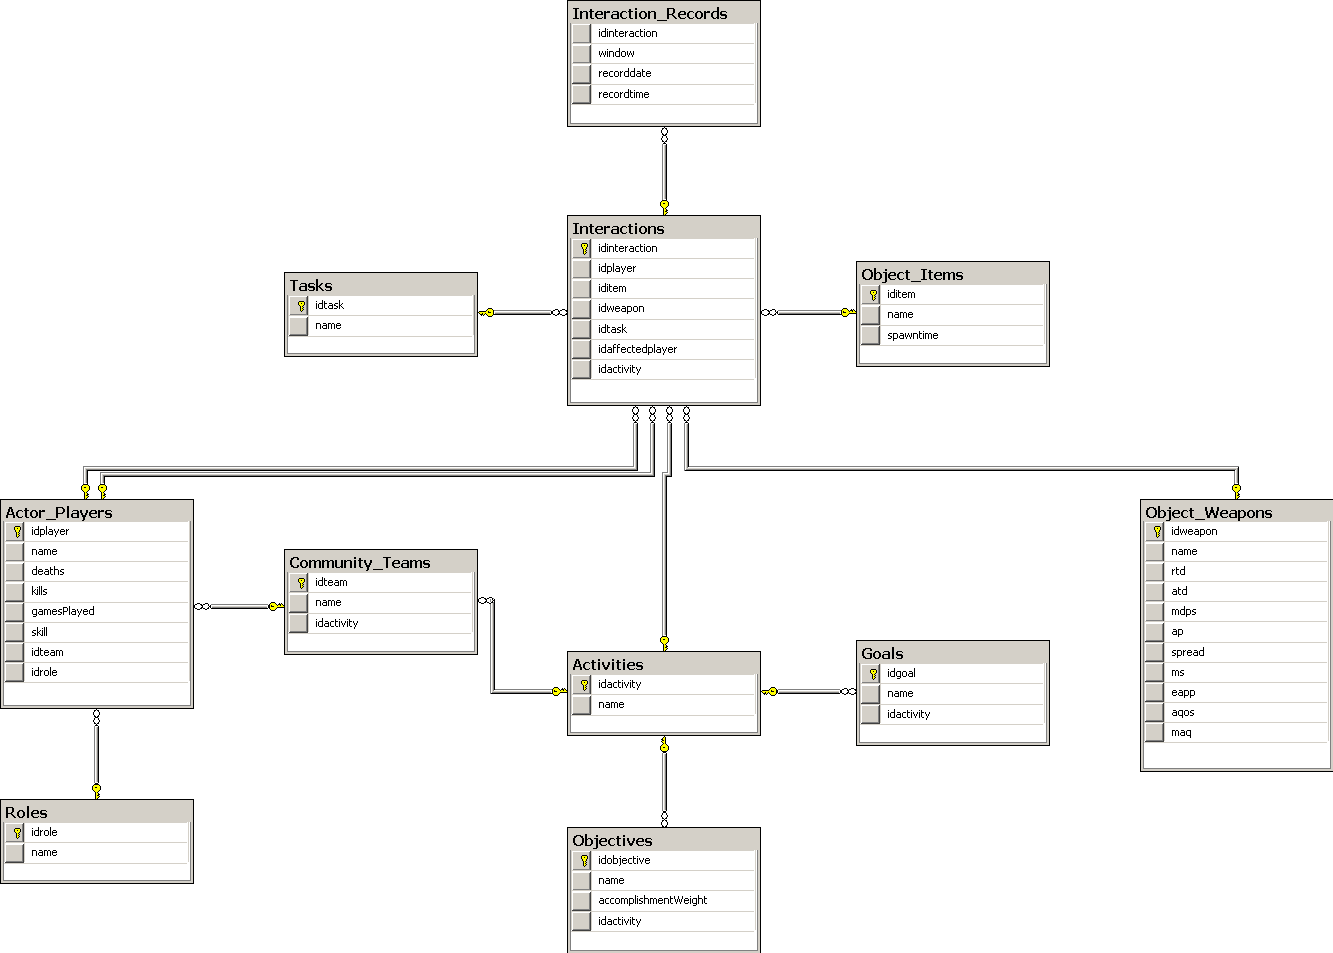
\includegraphics[width=0.7\linewidth]{./images/GameModelDiagram}
\caption[Modelo de dominio de \textit{Assault Cube}]{}
\caption{}
\label{fig:DomModel}
\end{figure}


A partir de estos elementos pueden empezar a definirse algunas reglas, por ejemplo establecer una regla que diga que si un jugador captur\'o una bandera y est\'a en peligro inminente de ser atacado, el sistema muestre a sus compa\~neros de equipo la ubicaci\'on del abanderado y env\'ie una se\~nal de auxilio para que ellos puedan acudir a su ayuda.

Con estas interacciones y el conjunto de reglas definido se propone un conjunto de guiones que describen diferentes tipos de comportamiento dado el caso de estudio; entre los que se encuentra un guion para jugadores novatos, un guion para jugadores in\'utiles, uno para jugadores con comportamiento sospechoso que podr\'ian considerarse como traidores y uno para jugadores expertos. Estos guiones servir\'an al momento de ejecutar  Los guiones se definen como sigue.

\textbf{Guion para jugador inactivo:}

\begin{tabular}{|p{10cm}|l|}
\hline \textbf{Regla} & \textbf{Frecuencia} \\
\hline $Actor(Player\{*\})-Task(Shot)$ & 3 \\
\hline \& $Actor(Player\{*\})-Task(Move)$ & 10 \\
\hline \& $Actor(Player\{*\})-Task(PickItem)$ & 5\\ 
\hline \& $Actor(Player\{*\}).enemyKills=0$ & no aplica\\
\hline\& $Actor(Player{*}).allyKills=0$ & no aplica\\
\hline\& $Actor(Player{*})-Task(captureFlag)$ & 1\\
\hline\& $Actor(Player{*}).socialPresense=bad$ & no aplica\\
\hline\& $Actor(Player{*}) \rightarrow Team(red)$  & no aplica\\
\hline \multicolumn{2}{l}{$:=$} \\
\hline $[Actor(Player\{*\})  \rightarrow Team(red)]-Task(sendWarningMessage, Object(UI\{messageConsole\})$ & no aplica\\
\hline

\end{tabular}

\textbf{Guion para jugador novato}

\begin{tabular}{|p{10cm}|l|}
\hline \textbf{Regla} & \textbf{Frecuencia} \\
\hline $Actor(Player\{*\}).enemyKills$ & 2\\
\hline \& $Actor(Player\{*\}).deads>2$ & no aplica\\
\hline \& $Actor(Player\{*\})-Task(Shot)$ & 5\\
\hline \& $Actor(Player\{*\})-Task(scoreCapturedFlag)$ & 1\\
\hline \& $Actor(Player\{*\})-Task(loseFlag)$ & 1\\
\hline \& $[Actor(Player\{*\}) \rightarrow Team(red)]-Task(Shot).Success = true$ & 5\\
\hline \& $[Actor(Player\{*\}) \rightarrow Team(red)]-Task(Shot).Dimension = positive$ & 5\\
\hline \multicolumn{2}{l}{$:=$} \\
\hline $[Actor(Player\{*\}) \rightarrow Team(red)]-Task(sendMessage, Object(UI\{messageConsole\})$ & no aplica\\
\hline
\end{tabular}

\textbf{Guion para jugador experto}

\begin{tabular}{|p{10cm}|l|}
\hline \textbf{Regla} & \textbf{Frecuencia} \\
\hline $Actor(Player\{*\}).enemyKills>5$ & no aplica\\
\hline \& $[Actor(Player\{*\}) \rightarrow Team(red)]-Task(Shot).Success = true$ & 5\\
\hline \& $[Actor(Player\{*\}) \rightarrow Team(red)]-Task(Shot).Dimension = positive$ & 5\\
\hline \& $[Actor(Player\{*\}) \rightarrow Team(red)]-Task(Destroy).Bearer = true$ & 1\\
\hline \& $Actor(Player\{*\})-Task(captureFlag)$ & 3\\
\hline \& $Actor(Player\{*\}).socialPresence=quite good$ & no aplica\\
\hline \& $Actor(Player\{*\}).deads<2$ & no aplica\\
\hline\multicolumn{2}{l}{$:=$}\\
\hline $[Actor(Player\{*\}) \rightarrow Team(red)]-Task(showPosition,Object(UI\{map,displayScreen\})$ & no aplica\\
\hline \& $[Actor(Player\{*\}) \rightarrow Team(red)]-Task(sendHelpMessage,Object(UI\{messageConsole\})$ & no aplica\\
\hline
\end{tabular}

\textbf{Guion de jugador traidor}

\begin{tabular}{|p{10cm}|l|}
\hline $Actor(Player\{*\})-Task(captureFlag)$ & 1\\
\hline \& $[Actor(Player\{*\})\rightarrow Team(red)]-Task(Shot)-Affects([Actor(Player\{*\})->Team(red)])$ & 3\\
\hline \& $Actor(Player\{*\}).socialPresence = bad$ & no aplica\\
\hline \& $Actor(Player\{*\}).allyKills > 2$ & no aplica\\
\hline \& $[Actor(Player\{*\})\rightarrow Team(red)]-Task(Shot).Dimension = negative$ & 5\\
\hline \& $[Actor(Player\{*\})\rightarrow Team(red)]-Task(Shot).Dimension = positive$ & 1\\
\hline \multicolumn{2}{l}{$:=$}\\
\hline $[Actor(Player\{*\})\rightarrow Team(red)]-Task(blockWeaponry)-Affects([Object(Weapon\{*\})->Actor(Player\{*\})])$ & no aplica\\
\hline \& $[Actor(Player\{*\})\rightarrow Team(red)]-Task(sendWarningMessage,Object(UI\{messageConsole\})$ & no aplica\\
\hline
\end{tabular}
%%%%%%%%%%%%%%%%%%%%%%%%%%%%%%%%%%%%%%%%%%%%%%%%%%%%%%%%%%%%%%%%%%%%%%%%%555
\section{Prototipo}

En cuanto a la arquitectura, como se puede observar en la figura \ref{imp:Implementacion}, la arquitectura es implementada con dos servidores, SQL Server como motor de base de datos y Internet Information Services 7 (IIS7) Como Servidor web. Dentro del servidor de base de datos se encuentra el  meta modelo y las instancias de los modelos de dominio que se generen; dentro del servidor web se encuentran las aplicaciones necesarias para definir e instanciar los modelos y servicios necesarios para la ejecuci\'on de \textit{Assault Cube}

\begin{figure}[h]
\centering
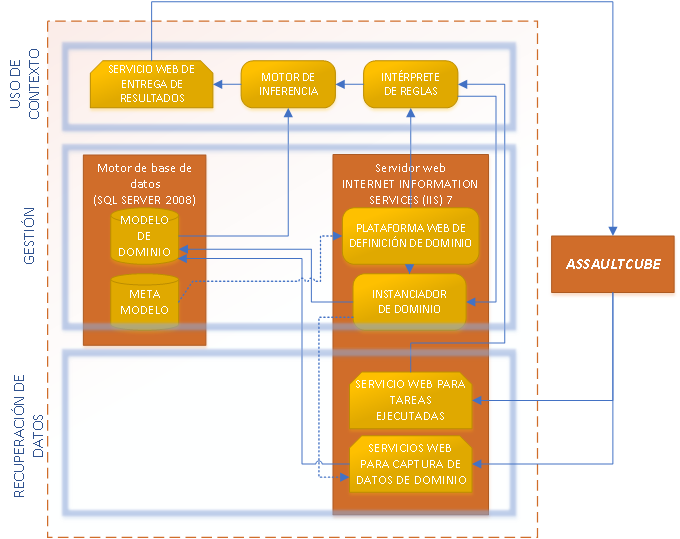
\includegraphics[width=0.7\linewidth]{./images/arquitecturaImplementacion}
\caption[Arquitectura de implementaci\'on]{}
\caption{}
\label{imp:Implementacion}
\end{figure}

